% CAPÍTULO 20 — «A janela que se escolhe sozinha» (a travessia: o tamanho decidido pelo dado)
% Fracasso que o abre: nenhuma escolha fixa serve aos dois mundos --- no que dobra, a janela de um
% ano erra por \numEsquecimentoJanelaDuzentosECinquenta{} do nível e a melhor fixa (cinquenta dias)
% erra por \numEsquecimentoJanelaCinquenta; no parado, a ordem se inverte. O sistema não sabe em que
% mundo está. Este capítulo mede se o dado pode escolher o tamanho sozinho.
% Caderno: E36_adaptativa (semente 103, \numAdaptativaMundos{} mundos, teste das metades, limiar
% orçado \numAdaptativaLimiarOrcado{} calibrado no parado).
% Figuras: figuras/E36_adaptativa_1.pdf (erro pós-degrau, cinco concorrentes) e
% figuras/E36_adaptativa_2.pdf (o tamanho ao longo do tempo, mundo com degrau e índice real).
% Costuras: o fecho do capítulo do esquecimento abre esta porta; o nosso fecho carrega a porta da
% ordem adiante, para o vigia da direção.

\chapter{A janela que se escolhe sozinha}\label{cap:escolhe}

\section{A pergunta que ninguém fez ao tamanho}

O capítulo do esquecimento terminou com a melhor memória medida e o seu número: no mundo que dobra
de uma vez, a janela de um ano erra por \numEsquecimentoJanelaDuzentosECinquenta{} do nível, a
melhor janela fixa --- cinquenta dias --- erra por \numEsquecimentoJanelaCinquenta, e a melhor
mistura exponencial, a memória de \numEsquecimentoMelhorMemoria{} dias, erra por
\numEsquecimentoMelhor. No mundo que não muda, a ordem se inverte: a janela longa quase não erra, e
as memórias curtas pagam o preço de sempre recomeçar. Cada número é a melhor escolha para um mundo
--- e o sistema não sabe em que mundo está.

A pergunta que falta é a do tamanho: pode o próprio dado escolher a janela, dia a dia, sem que
alguém declare o mundo antes? A literatura tem uma família para isso
\cite{gavalda2007learning,gama2004learning}, e ela cabe numa regra que cabe numa frase: guarde a janela, parta-a em duas, e
quando as metades discordarem além de um limiar, deixe a metade velha cair. O tamanho que sobra é o
que o dado escolheu. A pergunta deste capítulo é o preço dessa escolha --- medida na mesma moeda do
capítulo do esquecimento, porque é ela que a escolha fixa tem de bater.

\section{O teste das metades, declarado}

A janela guarda no máximo \numAdaptativaMaxima{} dias e nunca menos que \numAdaptativaMinima{} --- a
memória vencedora do capítulo anterior, para o estimador nunca ficar sem amostra. A cada dia, a
metade nova e a metade velha têm as suas médias comparadas; se a distância passa do limiar, a
metade velha cai, e o teste repete até as metades concordarem. A estimativa do dia é a média da
janela que sobrou. Os mundos são os do capítulo do esquecimento: \numAdaptativaDias{} dias, degrau
que dobra no dia \numAdaptativaQuandoMudanca{}, \numAdaptativaMundos{} mundos sorteados, tudo com a
dispersão entre eles junto.

O limiar é decisão, não ajuste. Ele é calibrado no mundo parado, antes de qualquer medição no mundo
que muda, contra um orçamento de encolhimentos falsos: quando nada muda, todo encolhimento é falso,
e a cadência desses falsos é contada por ano --- a mesma unidade em que o capítulo do orçamento do
alarme conta os seus alarmes no mundo parado. O orçamento declarado é um falso por ano no máximo, e
o limiar que o respeita é \numAdaptativaLimiarOrcado{}. E há o controle estrutural: com o limiar no
infinito, a janela que se escolhe sozinha é exatamente a fixa de \numAdaptativaMaxima{} dias, dia a
dia --- provado no teste do módulo, o análogo do controle de reação nula do capítulo do
instrumento. O que separa os dois é só o que o dado derrubou.

\section{O degrau: o dado escolhe a direção, não a escala}

\begin{table}[ht]
\centering
\caption{O erro relativo médio no ano seguinte à mudança, mediana entre mundos com a dispersão
entre parênteses. A janela que se escolhe sozinha fica na vizinhança da janela de um ano --- muito
acima da escolha certa para este mundo, muito abaixo do teto que ela seria sem encolher.}
\label{tab:escolhe_degrau}
\resizebox{\linewidth}{!}{%
\begin{tabular}{lcc}
\hline
concorrente & erro mediana & dispersão \\
\hline
janela de um ano & \numAdaptativaDegrauErroJanelaLongaMediana{} & (\numAdaptativaDegrauErroJanelaLongaDispersao) \\
janela de cinquenta dias & \numAdaptativaDegrauErroJanelaCurtaMediana{} & (\numAdaptativaDegrauErroJanelaCurtaDispersao) \\
mistura da memória de \numEsquecimentoMelhorMemoria{} dias & \numAdaptativaDegrauErroMisturaMediana{} & (\numAdaptativaDegrauErroMisturaDispersao) \\
o teto, sem encolher (\numAdaptativaMaxima) & \numAdaptativaDegrauErroTetoMediana{} & (\numAdaptativaDegrauErroTetoDispersao) \\
a que se escolhe sozinha & \numAdaptativaDegrauErroMediana{} & (\numAdaptativaDegrauErroDispersao) \\
\hline
\end{tabular}%
}
\end{table}

\begin{figure}[ht]
\centering
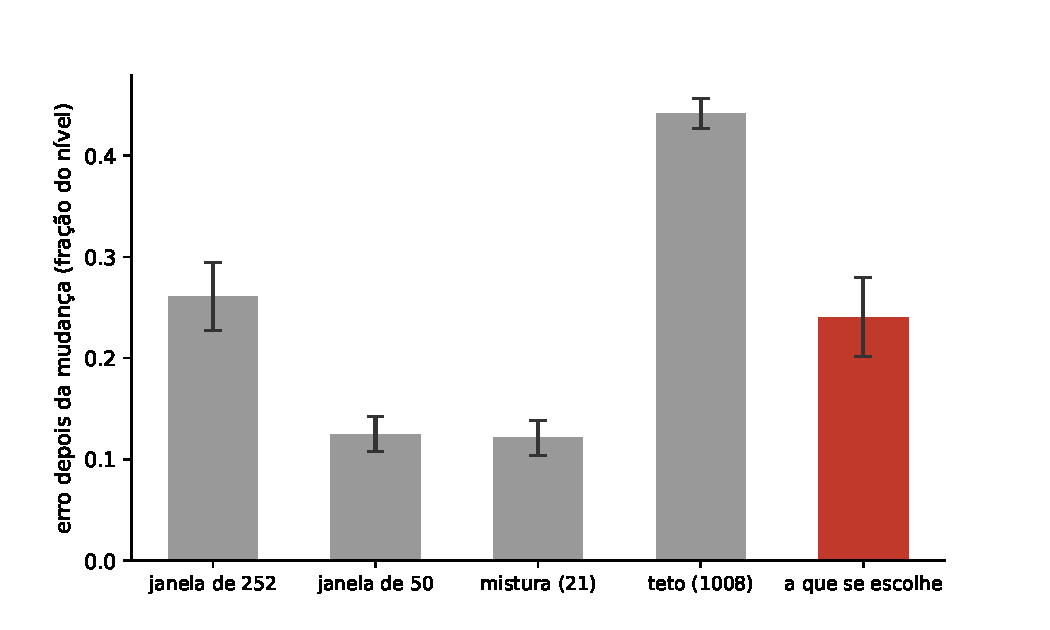
\includegraphics[width=\textwidth]{figuras/E36_adaptativa_1.pdf}
\caption{O erro no ano seguinte à mudança, cinco concorrentes, mediana e dispersão entre mundos. A
que se escolhe sozinha (vermelha) cai do teto para a vizinhança da janela de um ano --- e para ali
não desce: a escolha certa para este mundo, a janela de cinquenta dias, fica a mais de três
dispersões de distância.}
\label{fig:escolhe_degrau}
\end{figure}

O critério declarado era claro: recuperar a escolha certa sem saber o mundo. A medição diz que não.
O erro da janela que se escolhe sozinha é \numAdaptativaDegrauErroMediana, contra
\numAdaptativaDegrauErroJanelaCurtaMediana{} da janela de cinquenta dias --- mais de três dispersões
de distância. O que ela consegue é cair do teto: sem encolher, o erro seria
\numAdaptativaDegrauErroTetoMediana; encolhendo, ele cai para \numAdaptativaDegrauErroMediana, um
ganho de quase o dobro, e a deixa estatisticamente empatada com a janela de um ano. O dado escolheu
a direção --- fugir do passado que não vale mais --- e não escolheu a escala: a paridade é com a
janela que a pergunta do capítulo anterior já tinha medido como insuficiente para este mundo.

A razão está na escala do limiar, e olhá-la vale mais que o número. O limiar foi calibrado na
escala do mundo antigo --- o orçamento de falsos é contado onde nada muda. Quando o mundo dobra, o
ruído das metades dobra junto, e o mesmo limiar fica pequeno demais: a janela despenca na mudança
e não para mais de cortar --- \numAdaptativaDegrauEncolhimentosPorAno{} encolhimentos por ano no mundo
que dobrou, contra \numAdaptativaParadoFalsosPorAnoMediana{} falsos por ano no parado. Ela vive jovem:
tamanho médio de \numAdaptativaDegrauTamanhoMedioPos{} dias depois da mudança, vindo de
\numAdaptativaDegrauTamanhoAntes{} antes dela. E janela jovem em mundo barulhento é variação: a conta
fecha no mesmo lugar onde a janela de um ano fecha, não onde a escolha certa fecha.

\section{O preço no parado}

E quando nada muda, quanto custa deixar o dado escolher? O erro da janela adaptativa no mundo
parado é \numAdaptativaParadoErroAdaptativaMediana, contra \numAdaptativaParadoErroJanelaTetoMediana{}
do seu teto --- a diferença cabe numa dispersão entre mundos. A cadência de falsos fica em
\numAdaptativaParadoFalsosPorAnoMediana{} por ano na mediana (o pior mundo paga
\numAdaptativaParadoFalsosPorAnoPior), dentro do orçamento de um por ano que calibrou o limiar. A
escolha é quase grátis quando nada muda: é o seguro que este capítulo mede --- barato no parado,
insuficiente no degrau.

\section{As séries reais}

\begin{figure}[ht]
\centering
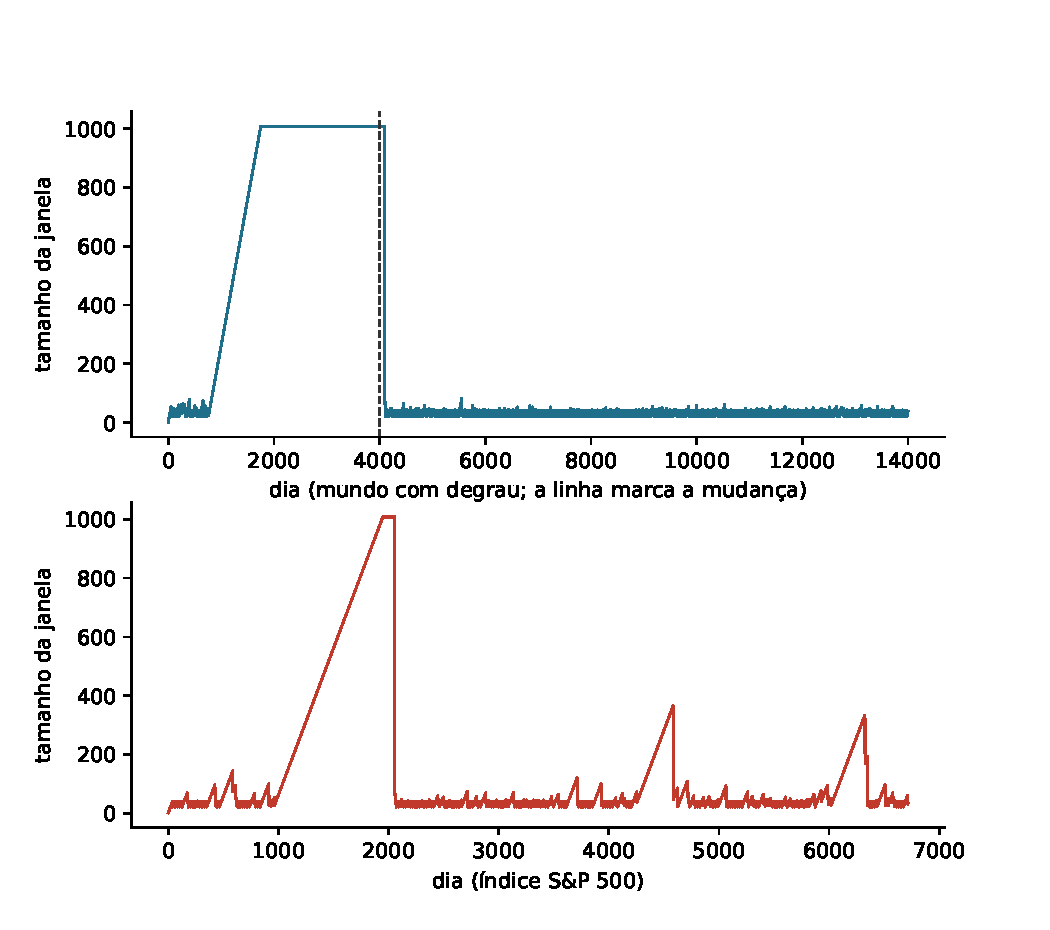
\includegraphics[width=\textwidth]{figuras/E36_adaptativa_2.pdf}
\caption{O tamanho que o dado escolhe, dia a dia: acima, um mundo com degrau (a linha pontilhada
marca a mudança) --- a janela despenca do máximo e nunca mais envelhece: oscila rente ao chão declarado; abaixo, o
índice real --- a janela quase não consegue crescer, e termina colada perto do chão de
\numAdaptativaMinima{} dias.}
\label{fig:escolhe_tamanhos}
\end{figure}

Nas séries reais, com o mesmo limiar orçado, o dado pede corte muito mais do que o mundo parado: o
índice encolhe \numAdaptativaRealSpEncolhimentosPorAno{} vezes por ano, o Ibovespa
\numAdaptativaRealIbovEncolhimentosPorAno, o Bitcoin \numAdaptativaRealBtcEncolhimentosPorAno --- e
termina com a janela em \numAdaptativaRealSpTamanhoFinal{} dias no índice e
\numAdaptativaRealBtcTamanhoFinal{} no Bitcoin, colada no chão declarado. Isto é medida do
instrumento, não afirmação sobre o mundo: o que ela diz é que, para este teste com este
orçamento, o dado real nunca deixa a janela envelhecer.

\section{O que fica}

O capítulo abriu com a pergunta do tamanho e a fecha com o preço dela medido. A janela que se
escolhe sozinha, com o orçamento honesto de falsos calibrado antes de medir, não alcança a escolha
certa no mundo que dobra --- fica na vizinhança da janela de um ano, entre o teto que seria sem
escolher e a memória curta que este mundo pediria. Ganha quase de graça o mundo parado. E nas
séries reais vive cortando. A conta que sobra é a de sempre: quem escolhe o tamanho escolhe o que
jogar fora --- e o que o esquecimento joga fora junto com os dias velhos é a \textbf{ordem} em que
eles vieram. É a ordem que diz para onde o tempo aponta, e é essa a pergunta seguinte.